\chapter{Planification des trajectoires}


\section{Introduction}

Dans les précédents chapitre ont présentés des lois de commandes qui calculent les commandes à envoyer aux actionneurs pour obtenir soit des positions, des vitesses, des accélérations ou des forces désirée. Certaines loi de commandes nécessitait seulement une position finale cible alors que pour d'autre nous devions spécifier une position, une vitesse et une accélération en tout temps sur une trajectoire cible. Plusieurs tâches en robotique nécessite donc une couche intermédiaire entre des spécifications à haut niveau pour une tâche et les références qui doivent être fournit à une boucle de commande à bas niveau, cette étape intermédiaire est appelée la planification de trajectoire.

\video{Introduction à la planification de trajectoires}{https://youtu.be/_SQumKYdFnM}
%TODO: Refaire une introduction plus générique

\paragraph{Pourquoi donner directement la position finale désirée à un contrôleur bas niveau en position n'est pas toujours approprié?}
L'étape de planification de trajectoire est généralement essentiel lorsqu'un robot doit faire un mouvement de grande amplitude, i.e. lorsque la position cible est éloignée de la position actuelle. Les loi de commandes bas-niveau sont typiquement conçu pour garantir la convergence vers la position cible mais pas le détail du chemin pour s'y rendre ni la vitesse d'approche; plus la cible est loin, plus il va y avoir de raison de mieux contrôler les étapes intermédiaire pour ce rendre à la cible. Voici une liste non-exhaustive de raisons pour mieux contrôler le trajet jusqu'à une cible:
\begin{enumerate}
    \item \textbf{Obstacles et contraintes en position:} Parfois il y a des positions/configurations sur lesquelles on ne veux pas que le système robotique ce retrouve (collisions avec des obstacles, singularités, etc.). Les lois de commande simples vont typiquement allez directement droit vers la cible et possiblement la dépasser avant de se stabiliser sur celle-ci sans tenir compte de contraintes. Un planificateur de trajectoire peut déterminer un chemin à suivre pour atteindre la cible qui évite des obstacles et positions inadéquates.
    \item \textbf{Contraintes en vitesse:} Les contrôleurs simples vont typiquement aller vers la cible avec une vitesse proportionnelle avec l'erreur initiale sans tenir compte des limites physiques. Si des saturations à bas niveau font que la vitesse réelle ne suit pas la vitesse commandée le comportement et la convergence de la loi de commande seront incertains. De plus, pour des raisons de sécurité il peut être nécessaire de limiter la vitesse d'un robot. Un planificateur de trajectoire peut déterminer un profil de vitesse à suivre qui respecte des contraintes.
    \item \textbf{Faisabilité dynamique:} Finalement, surtout pour des robots dynamiques et/ou qui bougent rapidement, les lois de commande de base peuvent facilement se retrouver dans des situations ou ils demande des niveaux d'accélération ou de forces aux actionneurs qui se sont pas physiquement possible. Un planificateur peut permettre de déterminer une séquence d'action physiquement possible qui vont mener le robot jusqu'à la cible tout en respectant des contraintes.
\end{enumerate}

%TODO: Demo colab pendule swing-up avec et sans trajectoire cible



\section{Chemin et profil temporel}
\label{sec:chemin}

\note{Système de coordonnées pour définir une trajectoire}{On peut définir des trajectoires dans plusieurs systèmes de coordonnées. Toutefois, pour simplifier la notation, nous présenterons ici d'abord plusieurs concepts en considérant que le trajet est toujours définit dans l'espace des joints d'un robot. Nous verrons ensuite que ces concepts se généralisent pour d'autres systèmes de coordonnées. }

Il est parfois utile d'utiliser le concept d'un chemin pour découpler le problème de planification de trajectoire en deux étapes: 1) trouver un chemin, une description géométrique d'une séquence de configuration $\col{q}$ reliant le point de départ et la cible; et ensuite 2) déterminer un profil temporel de vitesse sur ce chemin pour fixer une trajectoire temporelle.

\begin{figure}[htbp]
	\centering
		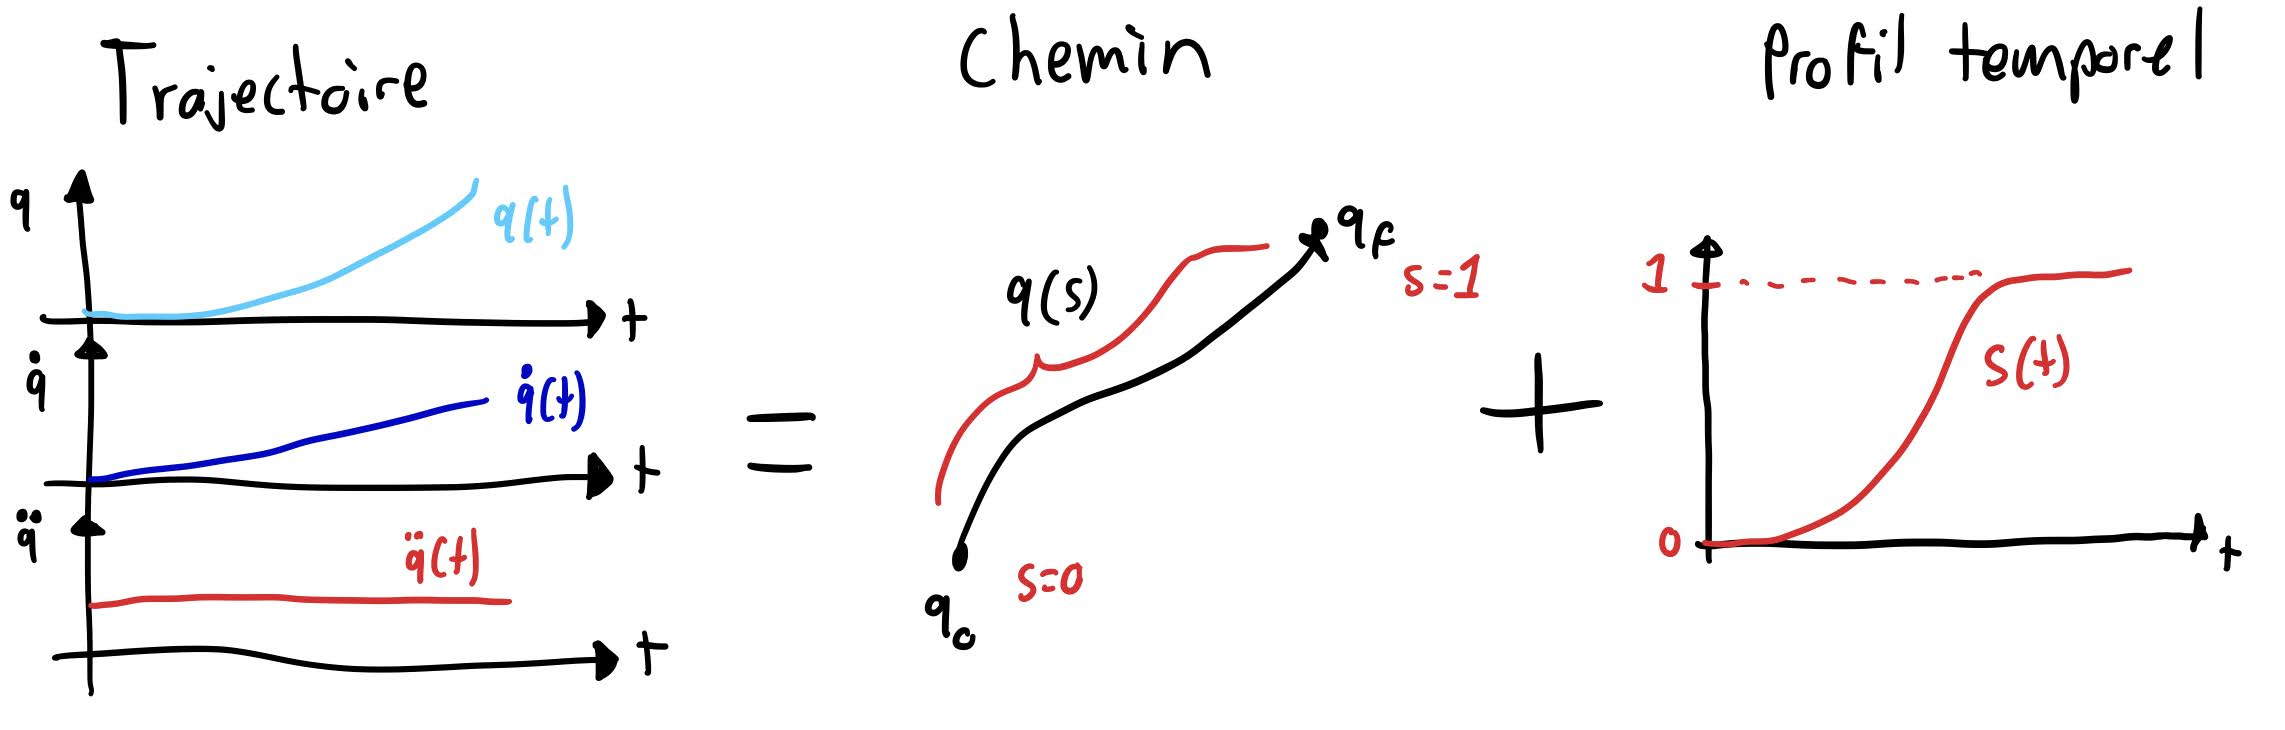
\includegraphics[width=0.90\textwidth]{fig/traj_path.jpg}
	\caption{Trajectoire (dans l'espace des joints), chemin et profil temporel}
	\label{fig:traj_path}
\end{figure}

\paragraph{Trajectoire} Une trajectoire est une fonction qui détermine la position d'un robot comme une fonction du temps $\col{q}(t)$. Normalement il est désirable d'avoir des fonctions qui sont dérivables deux fois, i.e. que la dérivé temporelle de cette fonction ne soit pas discontinue, ce qui impliquerait des accélérations d'amplitude infinie. La trajectoire est donc ultimement les trois fonctions suivantes:
\begin{align}
    \text{Trajectoire:} \quad \col{q}(t), \col{\dot{q}}(t), \col{\ddot{q}}(t) \quad \text{avec} \quad t \in [0,t_f]
\end{align}

\paragraph{Chemin} Une chemin est une fonction qui détermine la position d'un robot comme une fonction continue d'une variable scalaire $s \in [0,1]$, qui est égale à 0 au début du chemin et à 1 à la fin du chemin. 
\begin{align}
    \text{Chemin:} \quad \col{q}(s) \quad \text{avec} \quad s \in [0,1]
\end{align}

\paragraph{Profil temporel}  Un profil temporel est une trajectoire pour une variable scalaire intermédiaire qui caractérise la progression du système sur un chemin:
\begin{align}
    \text{Profil temporel:} \quad s(t), \dot{s}(t), \ddot{s}(t) \quad \text{avec} \quad t \in [0,t_f]
\end{align}

Lorsqu'on construit une fonction de trajectoire basé sur un chemin et un profil temporel on obtient les relations suivantes en appliquant une dérivée en chaîne :
\begin{align}
    \col{q}(t)       &=  \col{q}(s(t))\\
    \col{\dot{q}}(t) &= \frac{\partial \col{q}}{ \partial s}  \dot{s}    \\
    \col{\ddot{q}}(t)&= \frac{\partial \col{q}}{ \partial s}  \ddot{s} + \frac{\partial^2 \col{q}}{ \partial s^2}  \dot{s}^2
\end{align}


\subsection{Profils temporels}

Cette section présente quelques types de profils temporels qui sont typiquement utilisée pour générer des trajectoires.

\subsubsection{Profil temporel trapézoïdal}

Une profil de type trapézoïdal, voir Figure \ref{fig:trap_profile_speed}, est utilisé fréquemment pour la génération de trajectoires simples pour plusieurs types de système asservis en position. Ce profil permet d'inclure directement une limite en vitesse $v_{max}$ et une limite en accélération $a_{max}$, c'est le profile qui donne la trajectoire la plus rapide possible considérant ces deux contraintes. Il existe toutefois des profils temporels plus lisses sans discontinuités, voir les prochaines sections, ce qui peut être un avantage. Le profile trapézoïdal consiste en trois phases: une phase d'accélération avec $\ddot{s} = a_{max}$, une phase de croisière à vitesse constante avec $\dot{s} = v_{max}$ et une phase de décélération avec $\ddot{s} = -a_{max}$. Les profils de positions et d'accélérations associés sont illustrés à la Figure \ref{fig:trap_profile_speed_all}. 
%%%%%%%%%%%%%%%%%%%%%%%%%%%%%%%%%%%%
\begin{figure}[htbp]
	\centering
		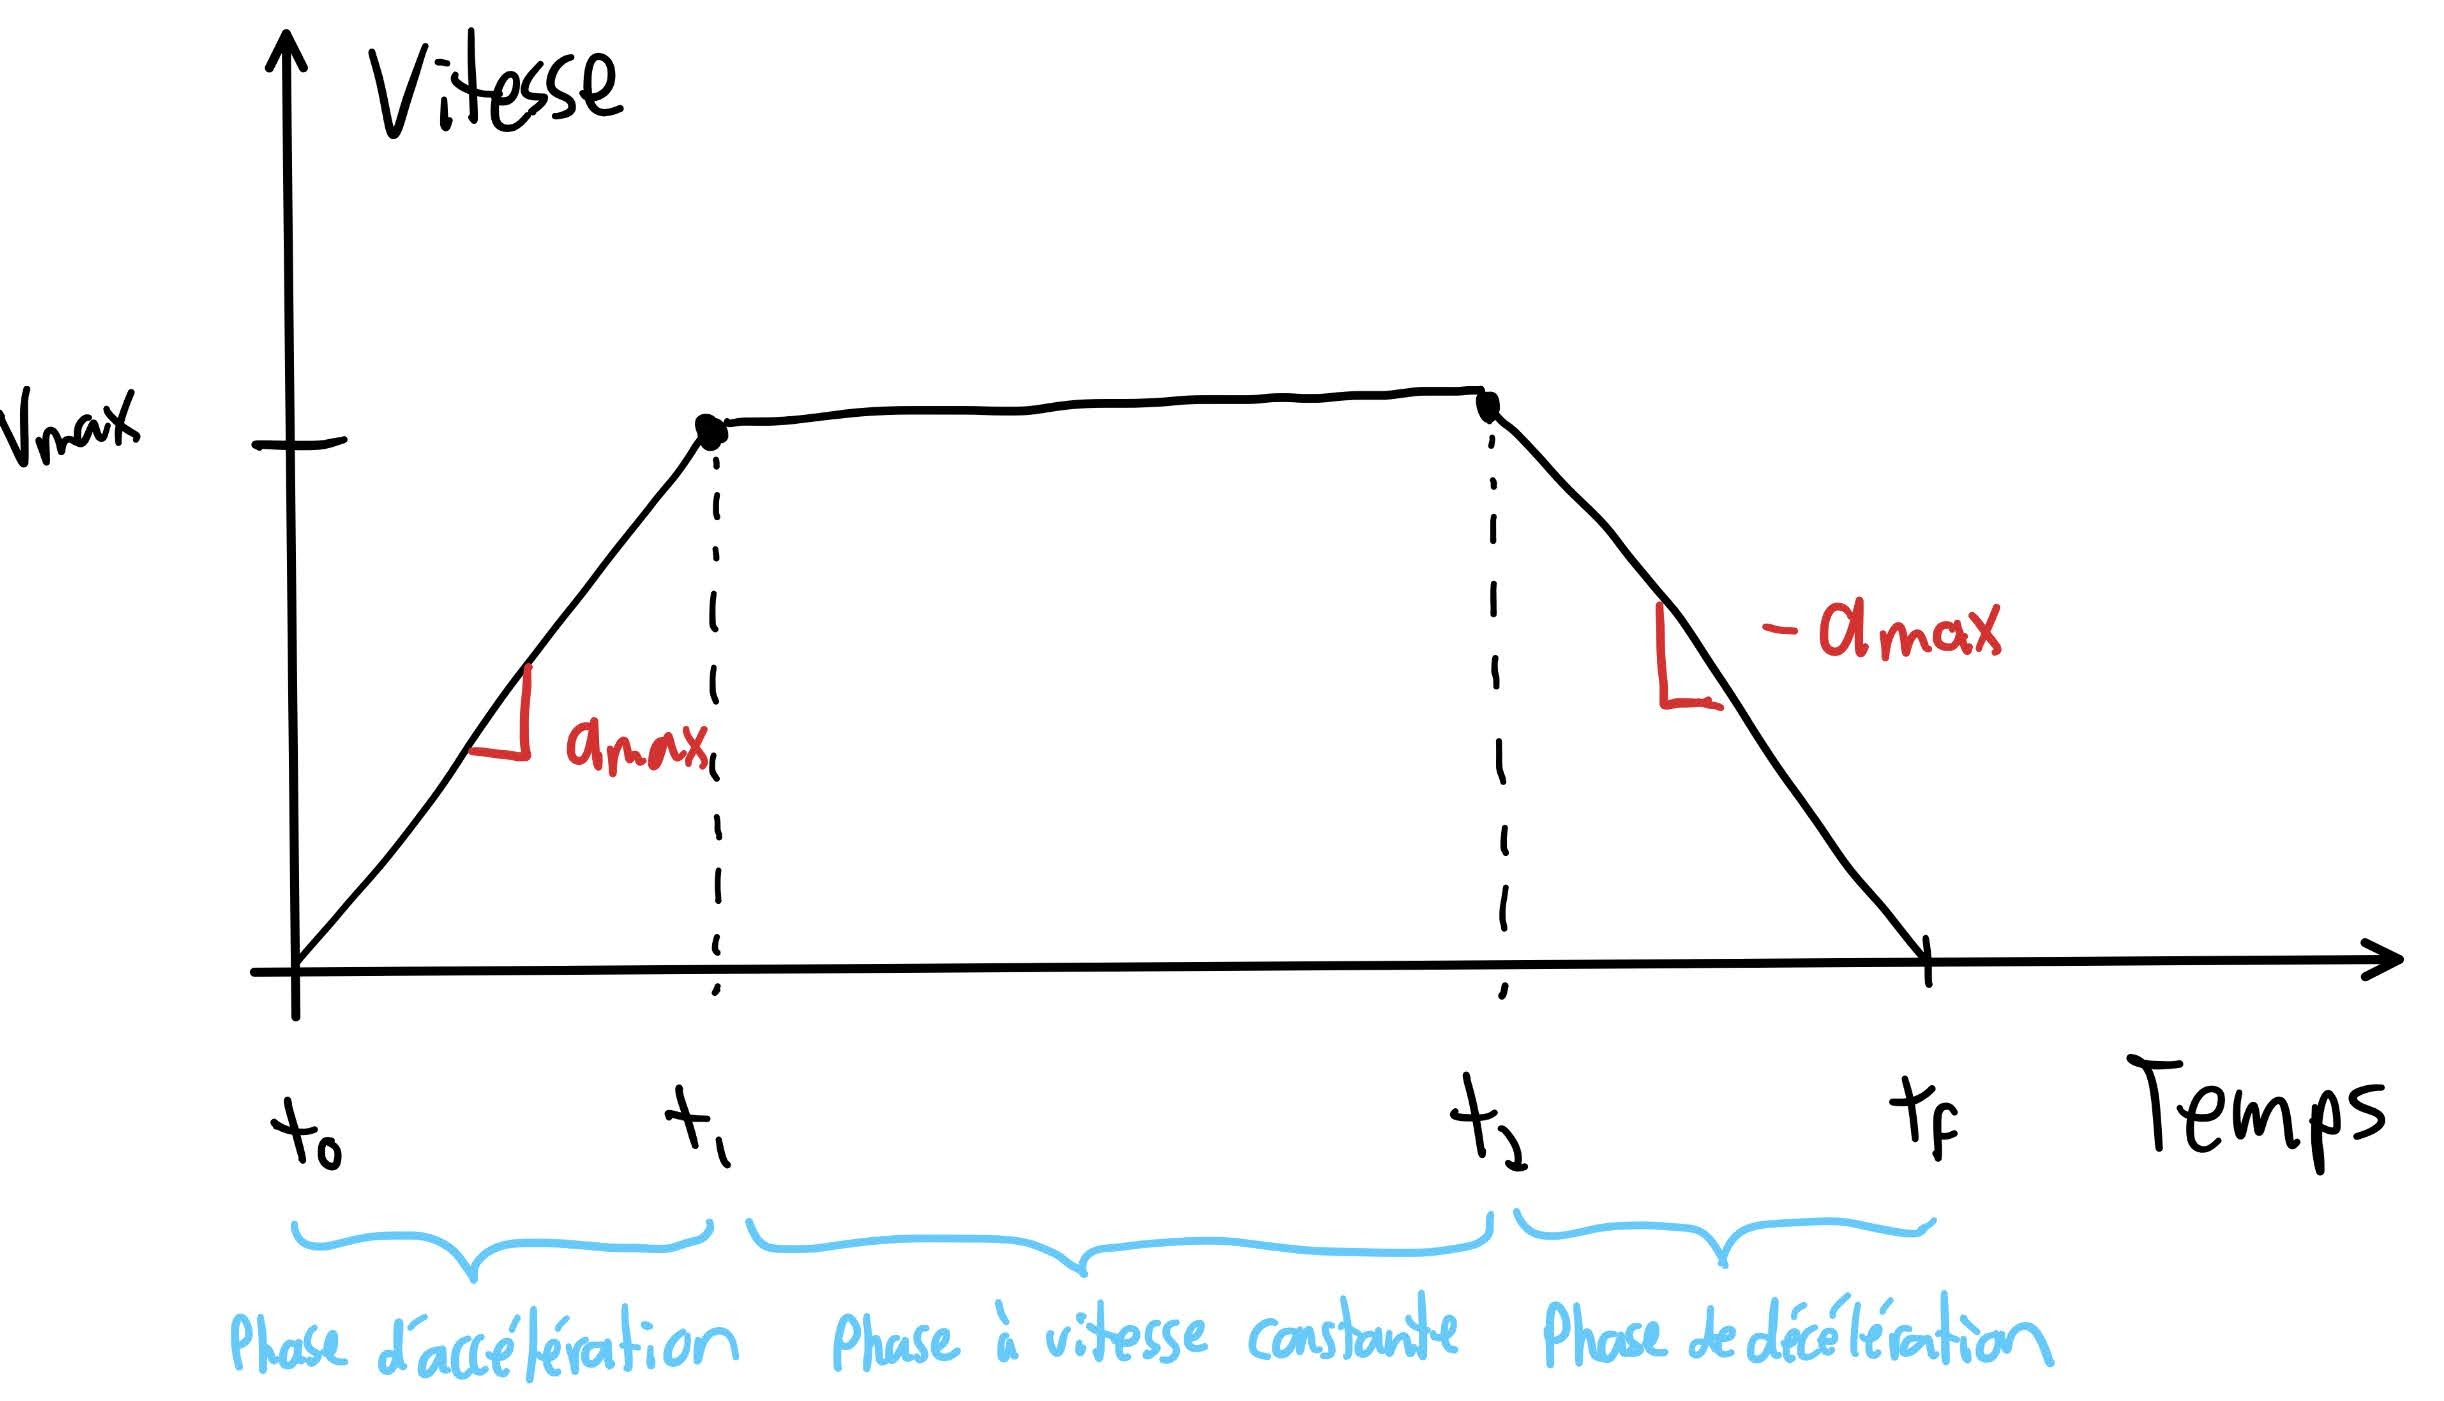
\includegraphics[width=0.70\textwidth]{fig/trap_profile_speed.jpg}
	\caption{Profil temporel de vitesse de type trapézoïdal}
	\label{fig:trap_profile_speed}
\end{figure}
%%%%%%%%%%%%%%%%%%%%%%%%%%%%%%%%%%%%

Si on utilise le concept de la variable $s$ qui représente la fraction du chemin à parcourir (voir section \ref{sec:chemin}), l'intégrale du profile de vitesse $\dot{s}(t)$ doit être égal à 1 (100\% du chemin parcouru). Il reste donc seulement trois variable, donc seulement deux sont indépendantes, pour définir complètement le profile temporel de $s(t)$: la vitesse maximale $v_{max}$, l'accélération maximale $a_{max}$ et la durée totale $t_f$ du trajet. Il peut être intéressant de déterminer les contraintes $v_{max}$ et $a_{max}$ du profile basé sur les limites physiques d'un système et ainsi obtenir la trajectoire qui minimise $t_f$:
%%%%%%%%%%%%%%%%%%
\begin{align}
t_f = \frac{a_{max}+v_{max}^2}{a_{max} v_{max}} 
\end{align}
%%%%%%%%%%%%%%%%%

Il est à noter que si $v_{max}^2/a_{max} > 1$ le système n'a pas le temps d'atteindre sa vitesse maximale de croisière et le profil est réduit à deux phases: accélération et décélération, voir Figure \ref{fig:trap_profile_triangle}.
%%%%%%%%%%%%%%%%%%%%%%%%%%%%%%%%%%%%
\begin{figure}[ht]
	\centering
		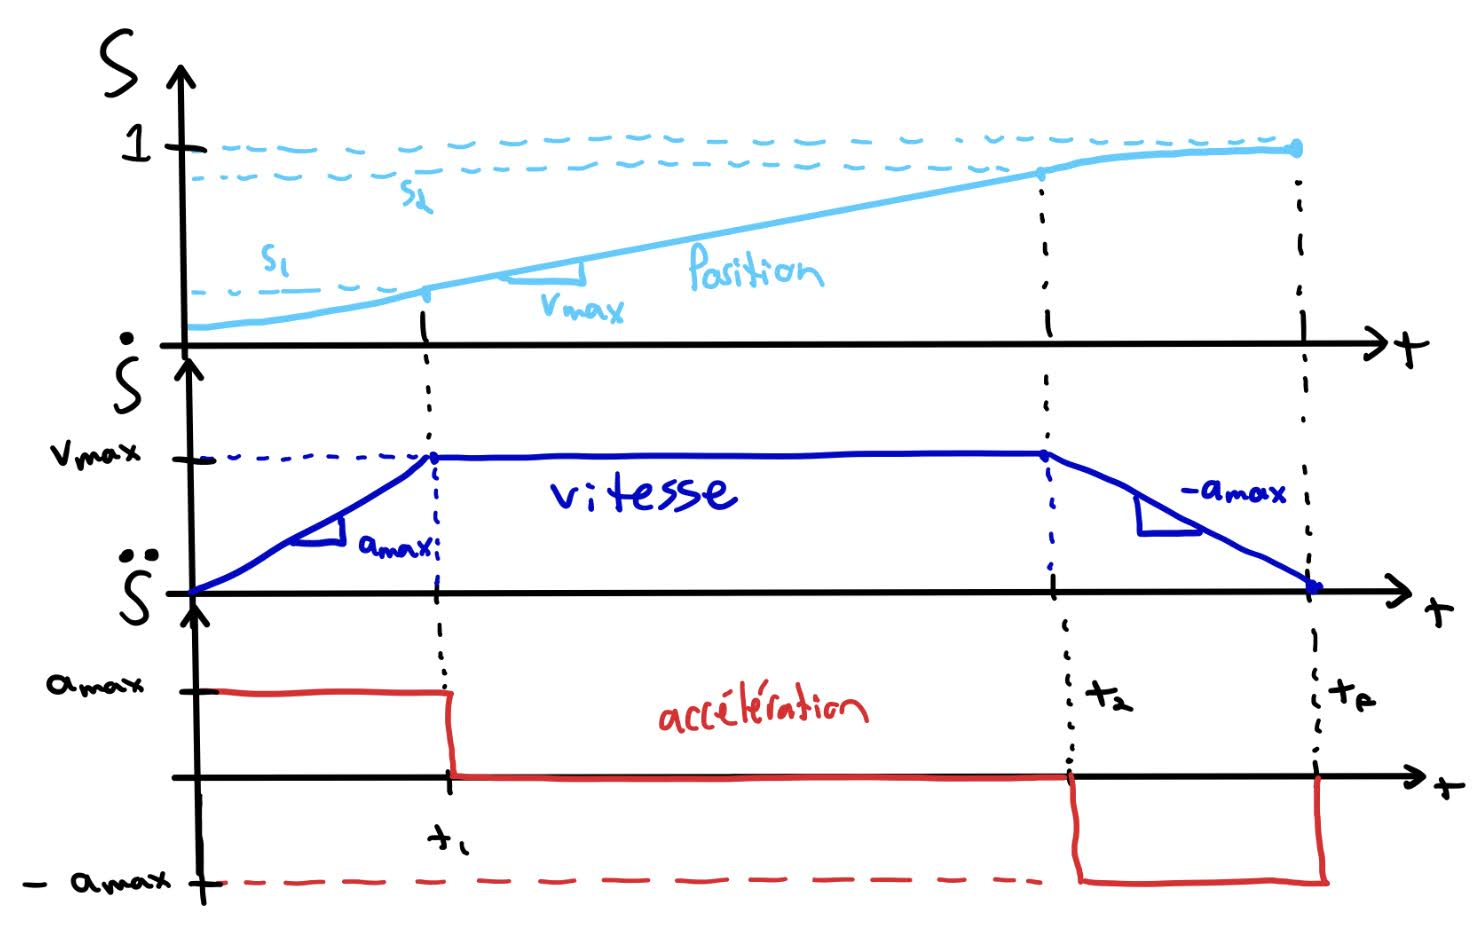
\includegraphics[width=0.70\textwidth]{fig/trap_profile_all.jpg}
	\caption{Position, vitesse et accélération pour un profil temporel de type trapézoïdal}
	\label{fig:trap_profile_speed_all}
\end{figure}
%%%%%%%%%%%%%%%%%%%%%%%%%%%%%%%%%%%%
%
Lorsque $v_{max}^2/a_{max}  \leq 1$, le profile est bien trapézoïdale et les équations de ce profile pour les trois segments temporels sont:
%%%%%%%%%%%%%%%%%%
\begin{align}
\text{si} \quad 0 \leq t \leq \frac{v_{max}}{a_{max}} \quad & \quad \left\{ \begin{array}{l}
s(t)= \frac{1}{2} a_{max} t^2
\\
\dot{s}(t)= a_{max} t
\\
\ddot{s}(t) = a_{max}
\end{array}
\right. \\
\text{si} \quad \frac{v_{max}}{a_{max}} < t \leq T- \frac{v_{max}}{a_{max}} \quad & \quad \left\{ \begin{array}{l}
s(t)= v_{max} t -  \frac{v_{max}^2}{2a}
\\
\dot{s}(t)= v_{max}
\\
\ddot{s}(t) = 0
\end{array}
\right. \\
\text{si} \quad  T- \frac{v_{max}}{a_{max}}  < t \leq T \quad & \quad \left\{ \begin{array}{l}
s(t) = \frac{2 a_{max} v_{max} T - 2 v_{max}^2 - a_{max}^2(t-T)^2}{2 a_{max}}
\\
\dot{s}(t)= a(T - t)
\\
\ddot{s}(t) = -a
\end{array}
\right.
\end{align}
%%%%%%%%%%%%%%%%%

%%%%%%%%%%%%%%%%%
\begin{figure}[ht]
	\centering
		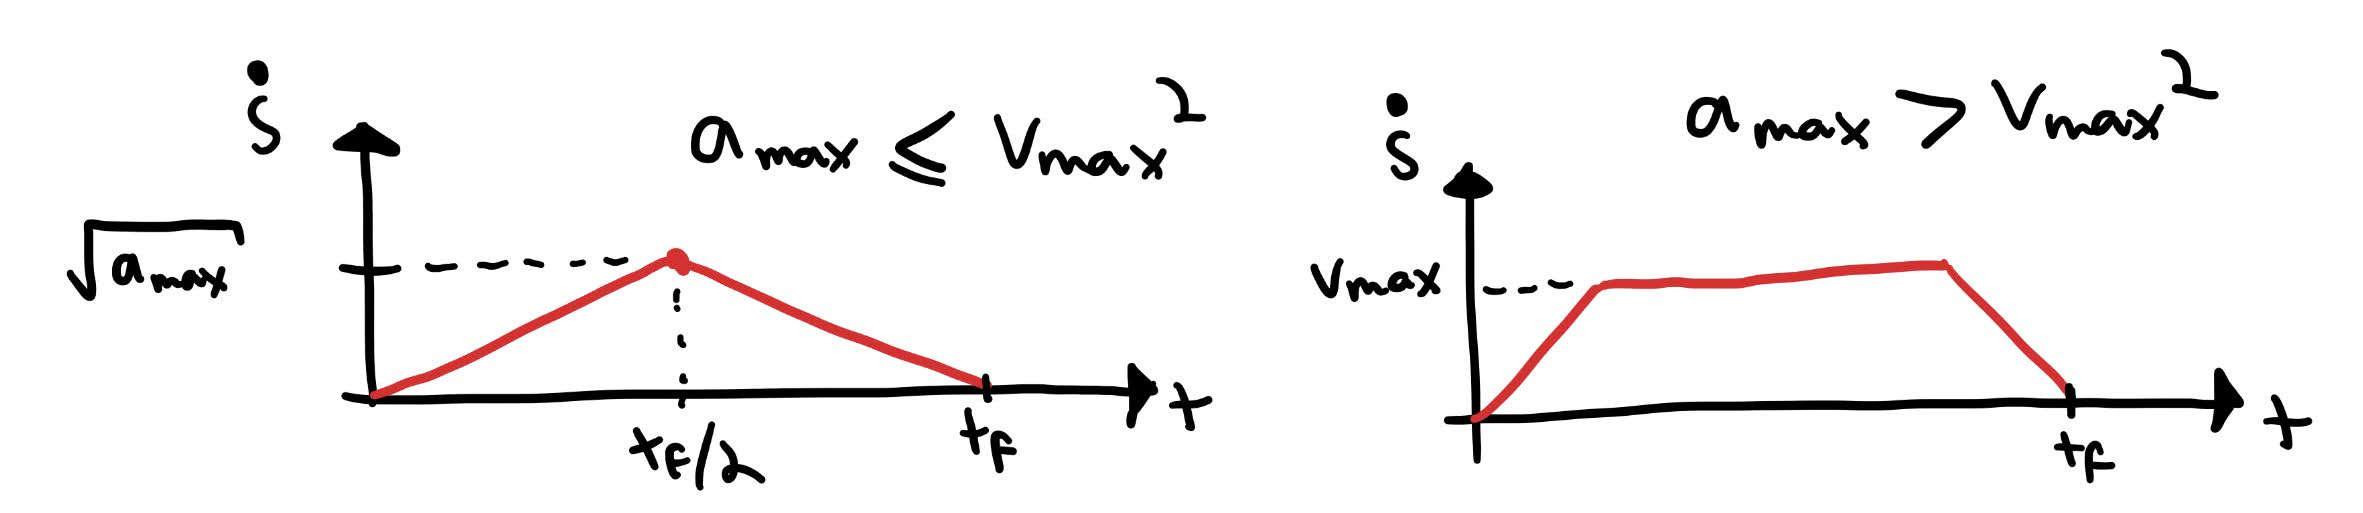
\includegraphics[width=0.80\textwidth]{fig/trap_profile_triangle.jpg}
	\caption{Cas limite du profile trapézoïdale}
	\label{fig:trap_profile_triangle}
\end{figure}
%%%%%%%%%%%%%%%%%





\subsubsection{Profil temporel polynomial d'ordre 3}

Une alternative à une profil temporel de type trapézoïdale est d'utiliser une fonction polynomiale. Pour obtenir un profile de vitesse qui débute à l'arrêt et termine aussi à l'arrêt, l'ordre minimum de la fonction est de trois. On obtient alors un profile de position cubique, un profile de vitesse parabolique et un profile d'accélération linéaire, avec comme équations:
%%%%%%%%%%%%%%%%%%
\begin{align}
s(t) &= a_0 + a_1 t + a_2 t^2 + a_3 t^3
\\
\dot{s}(t)&= a_1 + 2 a_2 t + 3 a_3 t^2
\\
\ddot{s}(t) &= 2 a_2 + 6 a_3 t 
\end{align}
%%%%%%%%%%%%%%%%%
Considérant que nous voulons représenter un mouvement qui débute et termine à l'arrêt, dans un temps $t_f$, nous avons les 4 contraintes suivantes à imposer: la position initial $s(0)=0$, la position finale $s(T)=1$, la vitesse initiale $\dot{s}(t_0)=0$ et la vitesse terminale $\dot{s}(t_f) = 0$. Il y a donc un seul paramètre libre, la durée du trajet $t_f$, et on peut trouver que:
%%%%%%%%%%%%%%%%%%
\begin{align}
a_0 = 0  \quad a_1 = 0  \quad a_2 = 3/t_f^2  \quad a_3 = -2/t_f^3 
\end{align}
%%%%%%%%%%%%%%%%%
ce qui donne comme équations de profile:
%%%%%%%%%%%%%%%%%%
\begin{align}
s(t) &=  \frac{3}{t_f^2}  t^2 -\frac{2}{t_f^3}  t^3
\\
\dot{s}(t)&= \frac{6}{t_f^2} t -\frac{6}{t_f^3}  t^2
\\
\ddot{s}(t) &= \frac{6}{t_f^2} -\frac{12}{t_f^3}  t 
\end{align}
%%%%%%%%%%%%%%%%%
qui sont illustrée à la Figure \ref{fig:poly3}.
%%%%%%%%%%%%%%%%%%%%%%%%%%%%%%%%%%%%%%%%%%%%%%%%%%%%%%%%%%%%%%%
\begin{figure}[ht]
				%\vspace{-10pt}
        \centering
				\subfloat[Ordre 3]{
				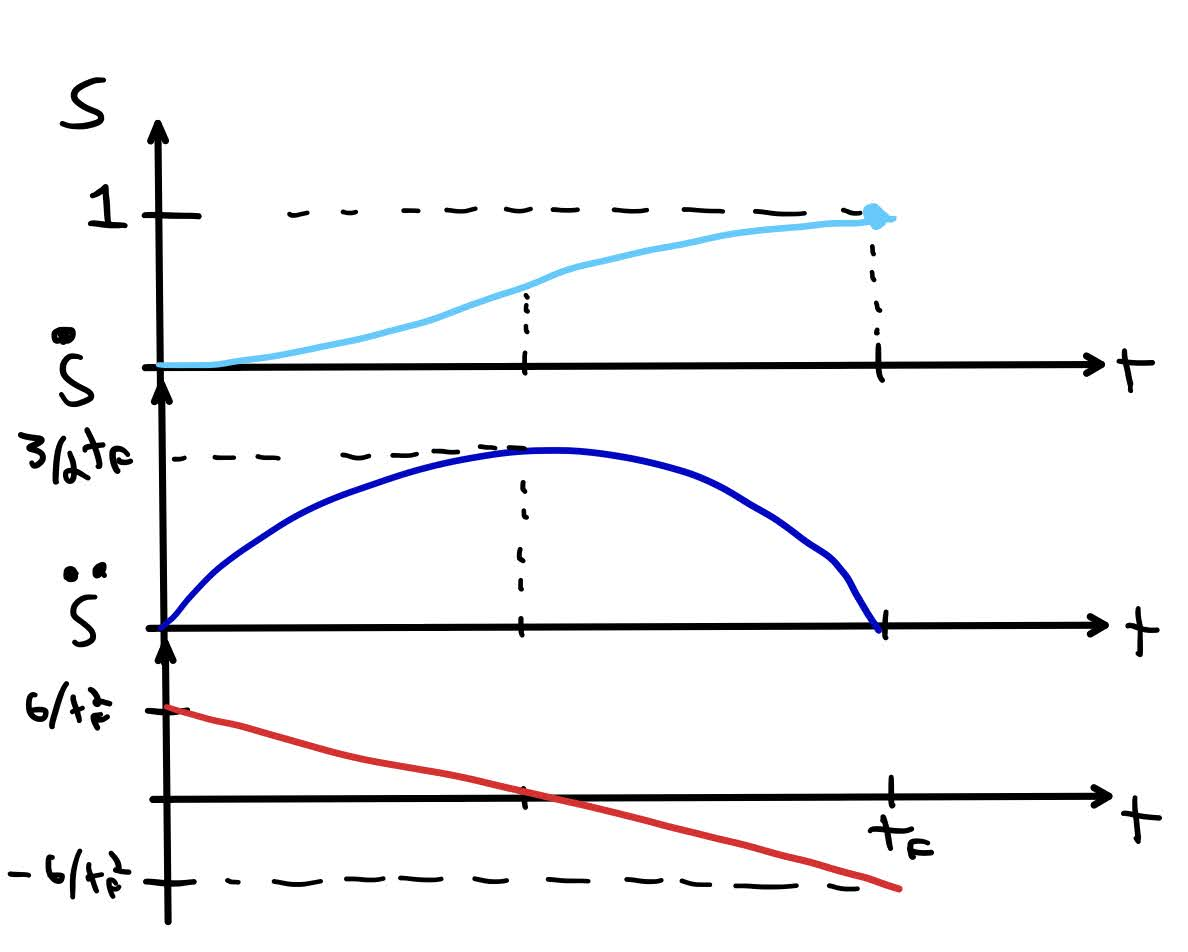
\includegraphics[width=0.49\textwidth]{fig/poly3_profile.jpg}
				\label{fig:poly3}}
				%%%%
				%\hspace{-5pt}
				%%%%
				\subfloat[Ordre 5]{
				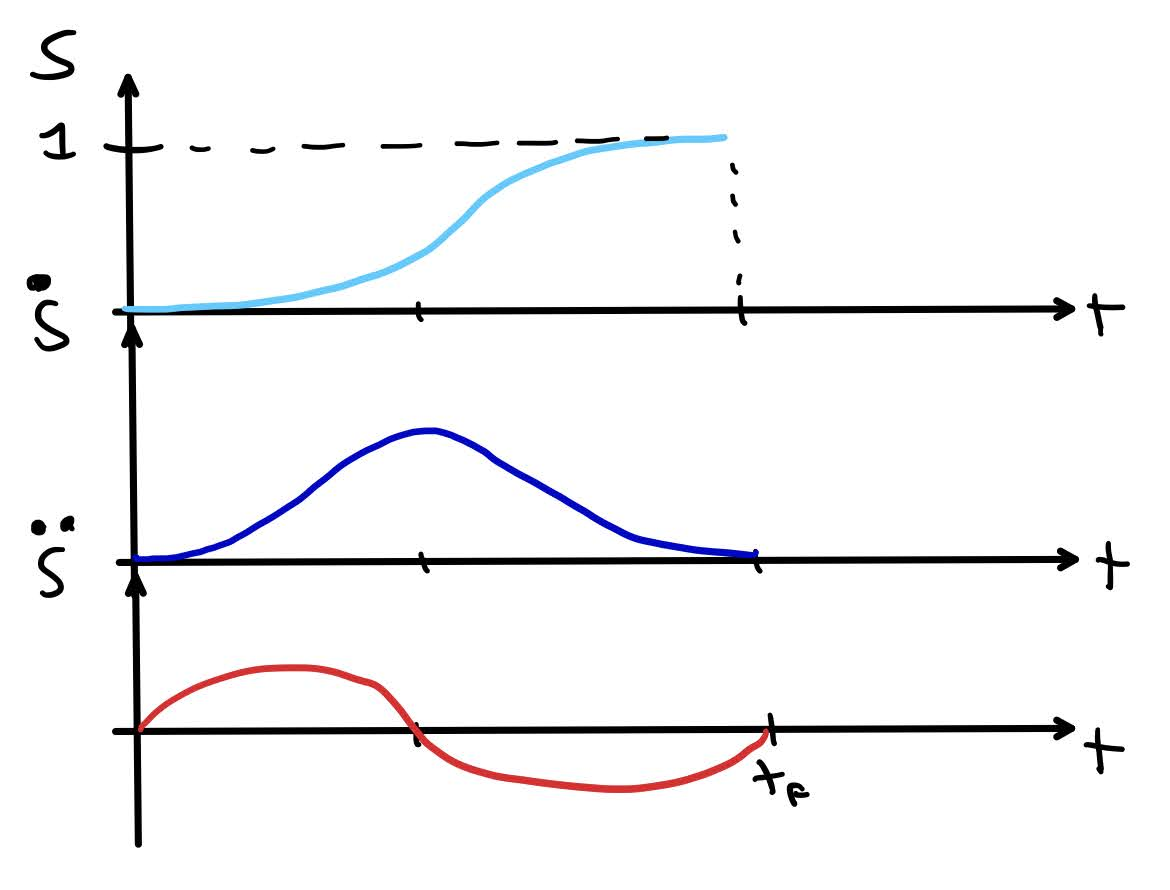
\includegraphics[width=0.49\textwidth]{fig/poly5_profile.jpg}
				\label{fig:poly5}}
        \caption{Profiles temporels polynonimaux}
			\label{fig:poly_profile}
\end{figure}
%%%%%%%%%%%%%%%%%%%%%%%%%%%%%%%%%%%%%%%%%%%%%%%%%%%%%%%%%%%%%%%%%

\subsubsection{Profil temporel polynomial d'ordre 5}

Une option pour avoir des trajectoires plus lisses est d'utiliser une fonction polynomiale d'ordre 5. Avec 5 paramètres il est possible de rajouter deux contraintes pour avoir une accélération qui débute et termine à une valeur de zéro, ce qui permet d'avoir aucune discontinuité en terme d'accélération, voir Figure \ref{fig:poly5} pour un allure de ce type de profile. Il est à noter que puisque nous avons rajouter 2 paramètres et 2 contraintes, comme pour le profile d'ordre 3 le profil d'ordre 5 a seulement $t_f$ comme paramètre libre. 


% \subsubsection{Courbe en S}

% À venir!

\newpage
\section{Planification cinématique pour les robots manipulateurs}

\subsection{Point à point dans l'espace des joints}

Si la position désirée d'un robot est déjà connue dans l'espace de ses joints, l'approche la plus simples est de générer un chemin linéaire dans l'espace des joints (voir Figure \ref{fig:traj_joint_line}) et ensuite d'ajuster le profil temporel en fonction des limites des actionneurs. L'objectif est donc de calculer des fonctions de trajectoires pour les joints en fonction d'une position actuelle, une position désirée et un temps de trajet:
%%%%%%%%%%%%%%%%%
\begin{align}
  \ddot{\col{q}}(t),\dot{\col{q}}(t),\col{q}(t) = plan(\col{q}_{0}, \col{q}_f, t_f)
	\label{eq:trajgen}
\end{align}
%%%%%%%%%%%%%%%%%
%%%%%%%%%%%%%%%%%
\begin{figure}[ht]
	\centering
		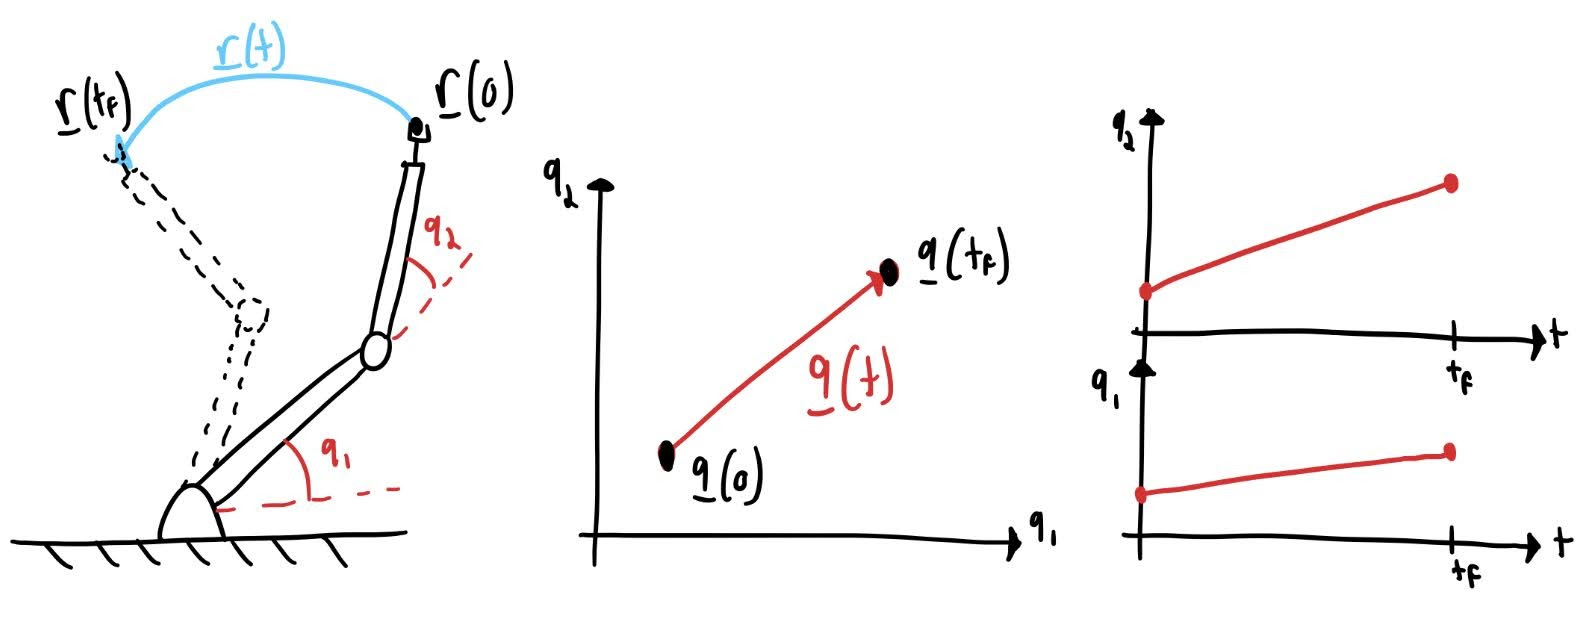
\includegraphics[width=0.80\textwidth]{fig/traj_joint_line.jpeg}
	\caption{Trajectoire en ligne droite dans l'espace de la tâche}
	\label{fig:traj_joint_line}
\end{figure}
%%%%%%%%%%%%%%%%

Un chemin en ligne droite dans l'espace des joints peut être défini par l'équation:
%%%%%%%%%%%%%%%%%
\begin{align}
  \col{q}(s) = \col{q}_0 + s ( \col{q}_f - \col{q}_0 )
\end{align}
%%%%%%%%%%%%%%%%%
On obtient alors comme dérivés:
%%%%%%%%%%%%%%%%%
\begin{align}
  \frac{\partial \col{q}}{ \partial s}  &= ( \col{q}_f - \col{q}_0 )
  \\
  \frac{\partial^2 \col{q}}{ \partial s^2} &= 0
\end{align}
%%%%%%%%%%%%%%%%%
et la relation entre les vitesses/accélérations des joints et le profil temporel est alors:
%%%%%%%%%%%%%%%%%
\begin{align}
  \col{\dot{q}} &= ( \col{q}_f - \col{q}_0 ) \dot{s}
  \\
  \col{\ddot{q}} &= ( \col{q}_f - \col{q}_0 ) \ddot{s}
\end{align}
%%%%%%%%%%%%%%%%%
Donc par exemple si on choisi un profil $s(t)$ trapézoïdale on peut choisir les paramètres $v_{max}$ et $a_{max}$ pour qu'ils correspondent avec les limites physiques des joints:
%%%%%%%%%%%%%%%%%
\begin{align}
  v_{max} \left( q_i(t_f) - q_i(0) \right)  \leq \max(\dot{q}_i) \quad \forall i
  \\
  a_{max} \left( q_i(t_f) - q_i(0) \right) \leq \max(\ddot{q}_i) \quad \forall i
\end{align}
%%%%%%%%%%%%%%%%%
ce qui correspond en fait simplement a ajuster pour l'amplitude du déplacement.

Planifier directement dans l'espace des joints a comme avantage de pouvoir vérifier intégrer directement les contraintes liés aux actionneurs (angles maximums, vitesses et accélérations). L'inconvénient c'est que la trajectoire de l'effecteur du robot n'est directement contrôlée.


\subsection{Point à point dans l'espace de la tâche}

Si la tâche se décrit mieux en termes de coordonnées cartésienne de l'effecteur par exemple, il est possible d'appliquer le même principe pour générer directement une trajectoire linéaire pour l'effecteur basé sur une position actuel, un position cible et un temps de trajet:
%%%%%%%%%%%%%%%%%
\begin{align}
  \ddot{\col{r}}(t),\dot{\col{r}}(t),\col{r}(t) = plan(\col{r}_{0}, \col{r}_f, t_f)
	\label{eq:trajgen}
\end{align}
%%%%%%%%%%%%%%%%%
%%%%%%%%%%%%%%%%%
\begin{figure}[ht]
	\centering
		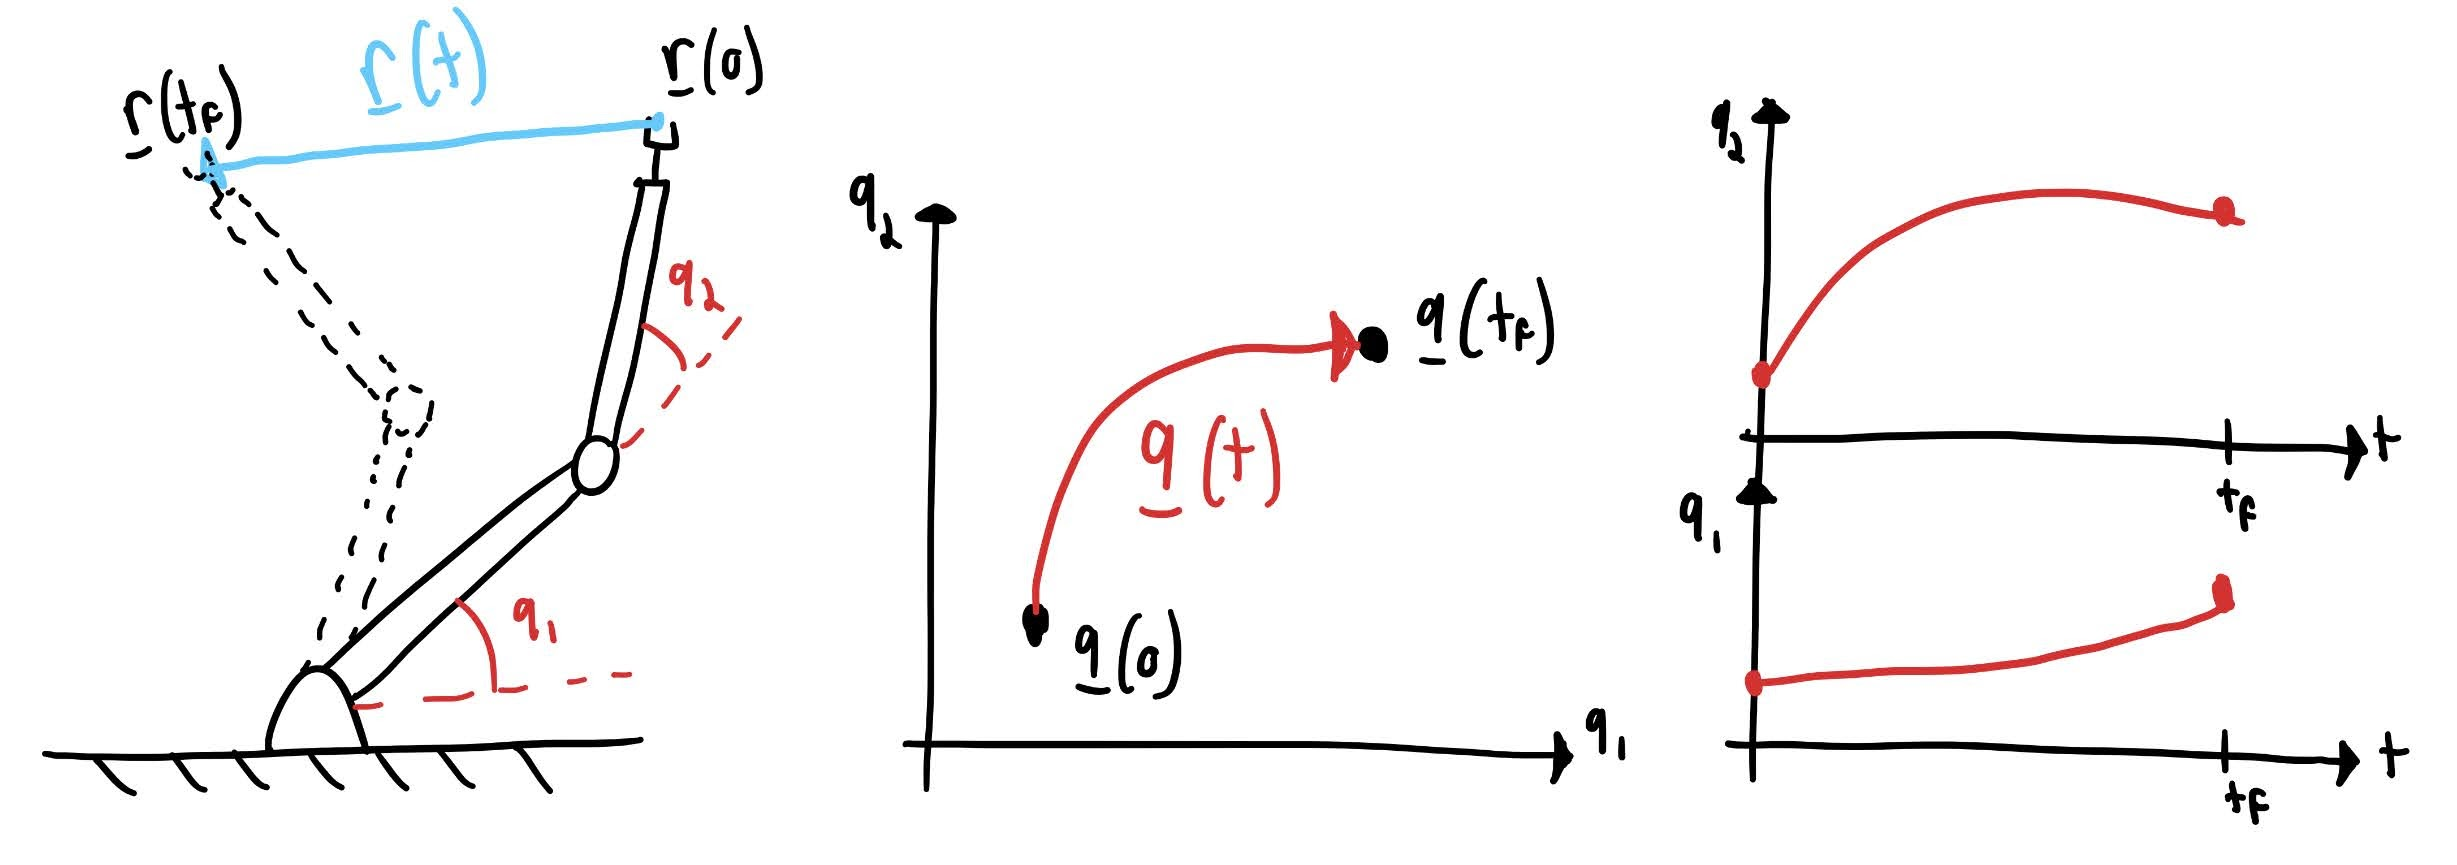
\includegraphics[width=0.80\textwidth]{fig/traj_eff_line.jpeg}
	\caption{Trajectoire en ligne droite dans l'espace de la tâche}
	\label{fig:traj_eff_line}
\end{figure}
%%%%%%%%%%%%%%%%%

Un chemin en ligne droite dans l'espace de la tâche peut être défini par l'équation:
%%%%%%%%%%%%%%%%%
\begin{align}
  \col{r}(s) = \col{r}_0 + s ( \col{r}_f - \col{r}_0 )
\end{align}
%%%%%%%%%%%%%%%%%
On obtient alors la relation suivante entre les vitesses/accélérations de l'effecteur et le profil temporel:
%%%%%%%%%%%%%%%%%
\begin{align}
  \col{\dot{r}} &= ( \col{r}_f - \col{r}_0 ) \dot{s}
  \\
  \col{\ddot{r}} &= ( \col{r}_f - \col{r}_0 ) \ddot{s}
\end{align}
%%%%%%%%%%%%%%%%%

Certaines approches de commande peuvent utiliser directement une trajectoire cible pour l'effecteur, par exemple la loi de commande cinématique présentée à la section \ref{sec:trajcontrol}, ou la loi de commande en impédance présentée à la section \ref{sec:effimpcontrol}. Alternativement, il est toujours possible de convertir la trajectoire de l'effecteur du robot dans l'espace des joints, avec un modèle cinématique (voir équation
\eqref{eq:ddj}), pour ensuite l'utilisée avec des lois de commande qui travaillent directement dans l'espace de joints.

Un inconvénient de planifier dans l'espace de la tâche est qu'on peut se retrouver dans des situations ou certains points intermédiaire du chemin sont hors de l'espace de travail du robot ou bien proche de singularité, même si le point de départ et la destination sont loin de configurations problématiques. Globalement, par rapport à l'approche d'envoyer directement la position cible dans une loi de commande, les méthodes point à point apportent seulement un meilleur contrôle du profile temporel. 

\subsection{Multi-points dans l'espace de la tâche}

Certaines tâches peuvent être décrites en termes de séquence de position à suivre, par exemple le code G pour des machines outils. Aussi, pour des problèmes de planification de chemin dans des environnements avec beaucoup d'obstacles, certains algorithmes de recherche vont retourner une séquence discrétisée de position à suivre pour le robot. Il y a donc plusieurs situations pour lesquels on doit générer une trajectoire basé sur un séquence de positions intermédiaires:
%%%%%%%%%%%%%%%%%
\begin{align}
  \ddot{\col{r}}(t),\dot{\col{r}}(t),\col{r}(t) = plan(\col{r}_{0}, \col{r}_{1}, \col{r}_{2}, ... , \col{r}_f, t_1, t_2, ... , t_f)
	\label{eq:trajgen}
\end{align}
%%%%%%%%%%%%%%%%%

\subsubsection{Segments}

L'approche la plus simpliste est d'utiliser la méthode point à point présentée à la section précédente pour chaque segment, voir Figure \ref{fig:traj_segments}. Toutefois, l'inconvénient majeur est que pour garantir qu'il n'y a aucune discontinuité dans les vitesses (ce qui mènerait à une accélération infinie), le robot doit s'immobiliser à tout les points où il y a des changements de directions. Ce n'est pas optimal ni en terme de consommation énergétique ni en terme de temps. 

%%%%%%%%%%%%%%%%%%%%%%%%%%%%%%%%%%%%%%%%%%%%%%%%%%%%%%%%%%%%%%%
\begin{figure}[ht]
				%\vspace{-10pt}
        \centering
				\subfloat[Segments]{
				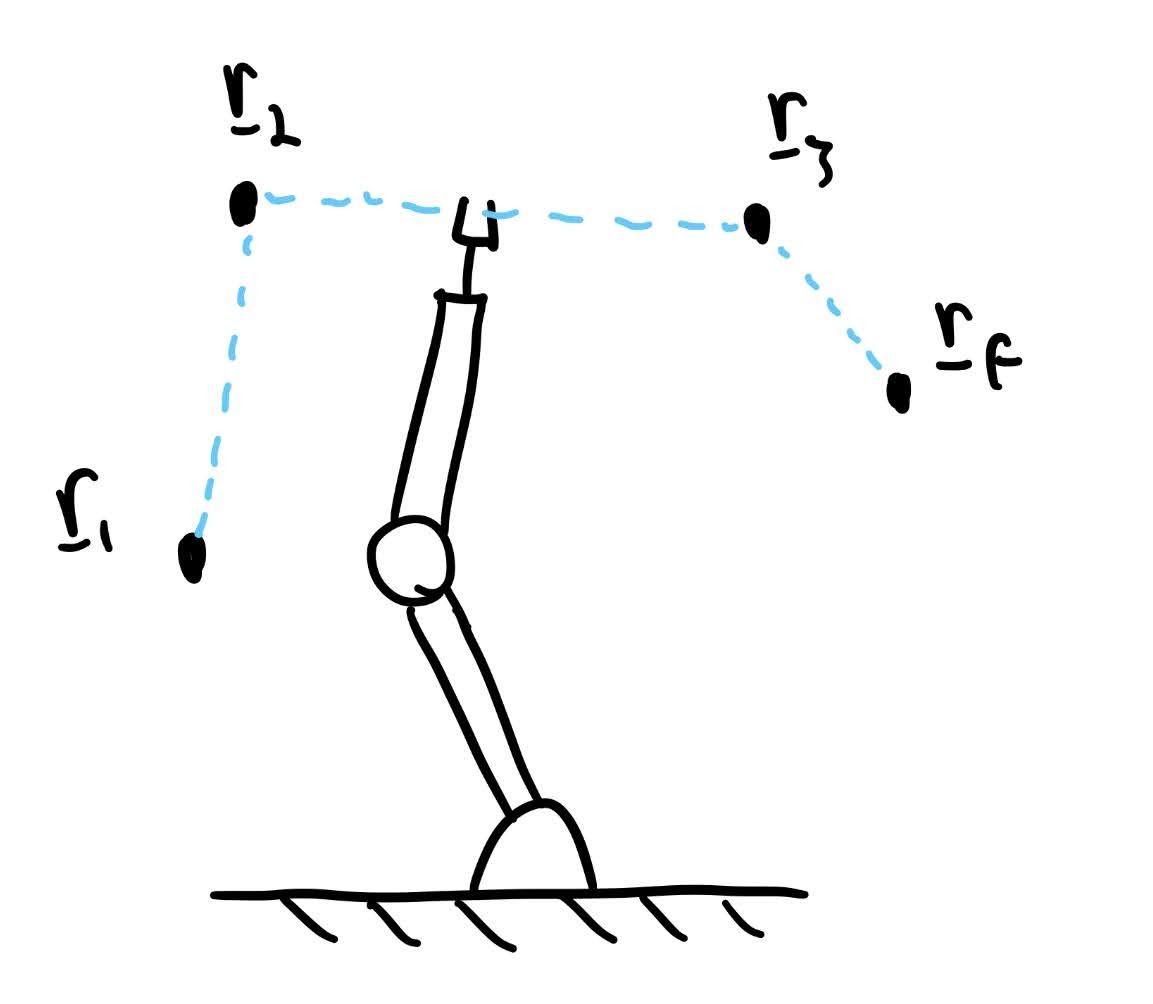
\includegraphics[width=0.49\textwidth]{fig/traj_segments.jpeg}
				\label{fig:traj_segments}}
				%%%%
				%\hspace{-5pt}
				%%%%
				\subfloat[Interpolation]{
				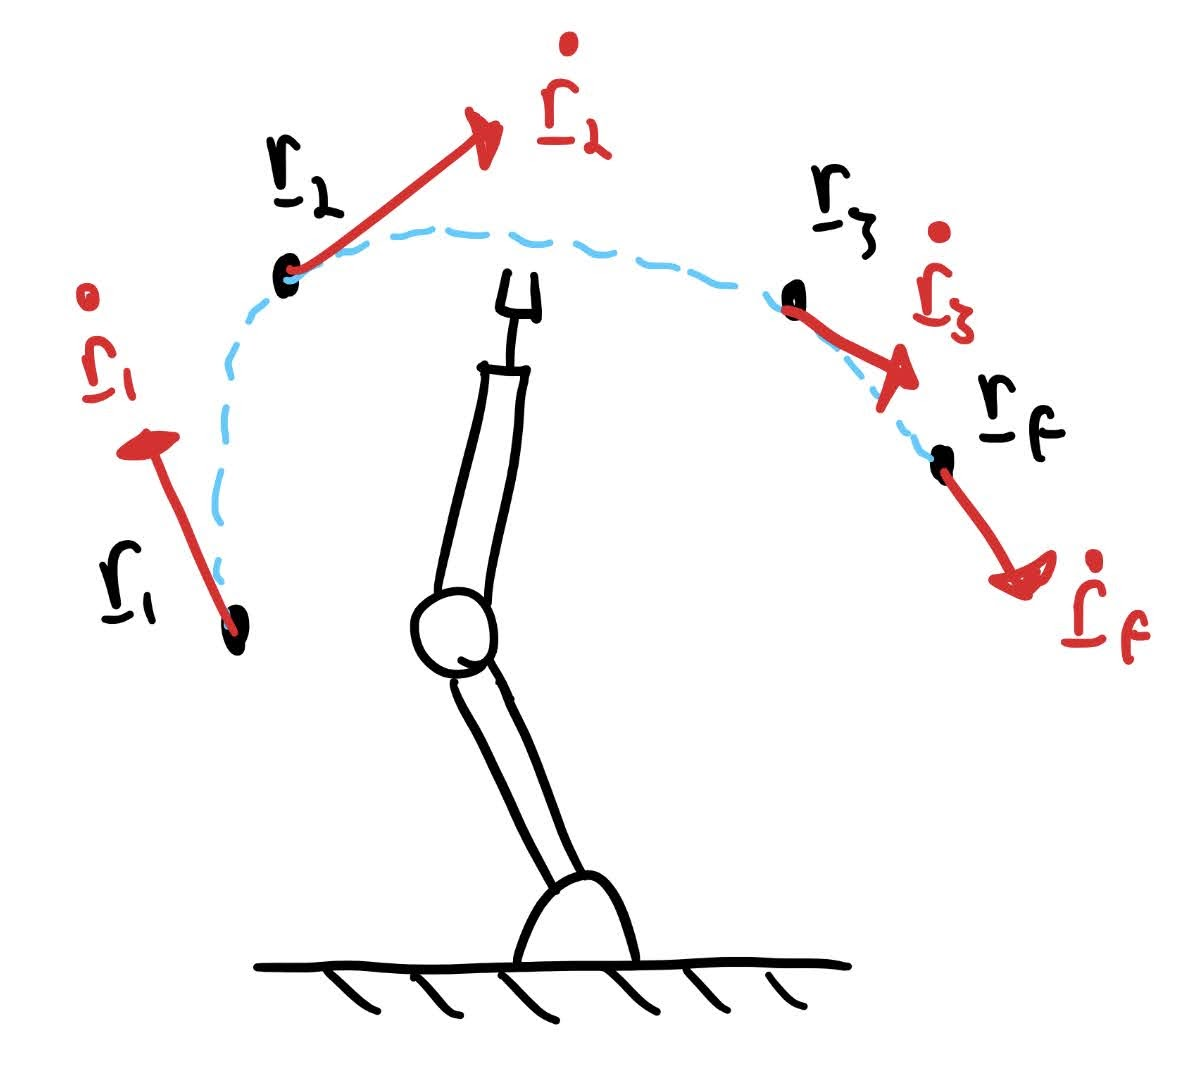
\includegraphics[width=0.49\textwidth]{fig/traj_interpol.jpeg}
				\label{fig:traj_interpol}}
        \caption{Trajectoire multi-points dans l'espace de la tâche}
			\label{fig:traj_multi_point}
\end{figure}
%%%%%%%%%%%%%%%%%%%%%%%%%%%%%%%%%%%%%%%%%%%%%%%%%%%%%%%%%%%%%%%%%


\subsubsection{Interpolation}

Une alternative est d'utiliser des fonctions d'interpolation pour générer une trajectoire plus lisse. Une approche est d'utiliser des polynômes cubique pour chaque segment, avec des contraintes de continuité en position et vitesse à chaque point intermédiaire. Il est aussi possible de spécifier des vecteurs de vitesses désirées à chaque point intermédiaire, qui peuvent être inclus comme des contraintes pour déterminer les paramètres des polynômes. Il existe plusieurs méthodes d'interpolation qui peuvent être utilisées pour ce type de problème, une autre méthode populaire est les \textit{B-spline}. 


\newpage
\section{Algorithmes d'optimisation de trajectoires}

\video{Introduction à la commande optimale}{https://youtu.be/3x6Vg-RRZ50}

\colab{Démo d'introduction à l'optimisation de trajectoires}{https://colab.research.google.com/drive/1yq2GHAkvO6fTF2W-tRbACDBa9_scec2k?usp=sharing}

À venir!

\section{Algorithmes de recherche}
\label{sec:searchalgo}

À venir!
